\documentclass[11pt,a4paper,roman]{scrartcl}
\usepackage{parskip}
\usepackage[english]{babel}
\usepackage{url}
\usepackage[utf8x]{inputenc}
\usepackage{amsmath}
\usepackage{amssymb}
\usepackage{graphicx}
\usepackage{listings}
\usepackage{float}
\usepackage{hyperref}
\usepackage[document]{ragged2e}
\usepackage{bm}
\usepackage[section]{placeins}
\title{Computer exercise 1}
\date{}
\author{Carl Ridnert, 940325-0112, ridnert@kth.se \\
Yue Jiao, 911024-7799, yj@kth.se}


\begin{document}
\maketitle
\begin{figure}[h]
\centering

\includegraphics[width=0.45\textwidth]{KTH_CMYK}
\end{figure}
\newpage
\section*{C.1.1.1}
In this subtask the following ODE shall be solved for different E, L, C, and R. 
\begin{equation}
L\ddot{q}+R\dot{q}+\frac{1}{C}q = E,\quad q(0)=0,\quad \dot{q}(0) = 0
\end{equation}

The desired solution is to rewrite the question in matrix form and it is done as follow. 
\begin{equation} \begin{aligned}
u_1 & = q \\ u_2 & = \dot{u_1} \\ L\dot{u_2} + R\dot{q}+\frac{1}{C}q & = E \\ 
& \Downarrow \\ \frac{du_1}{dt} & = u_2 \\
\frac{du_2}{dt} & = -\frac{1}{LC}u_1-\frac{R}{L}u_2+\frac{E}{L} \\ & \Downarrow \\
\begin{bmatrix} \frac{du_1}{dt} \\ \frac{du_2}{dt} \end{bmatrix} & = 
\begin{bmatrix} 0 & 1 \\ -\frac{1}{LC} & -\frac{R}{L} \\ \end{bmatrix} 
\begin{bmatrix} u_1 \\ u_2 \end{bmatrix} +
\begin{bmatrix} 0 \\ \frac{E}{L} \end{bmatrix} 
\end{aligned} \end{equation}

That is how the original equation is written in the form $\frac{d\vec{u}}{dt}=A\vec{u}+\vec{g}$. 
\begin{equation}
\begin{aligned}
A & = \begin{bmatrix} 0 & 1 \\ -\frac{1}{LC} & -\frac{R}{L} \\ \end{bmatrix} \\
\vec{g} & = \begin{bmatrix} 0 \\ \frac{E}{L} \end{bmatrix} 
\end{aligned}
\end{equation}

Then the ODE can be solved with the following formula: 
\[
\vec{u}(t) = e^{At}\vec{u_0} + A^{-1}(e^{At}-I)\vec{g}
\]

The numerical solutions are calculated by Matlab for different parameters. The results are plotted below as the values $q, \dot{q}, \ddot{q}$ for a certain amount of time. 

\begin{figure}[h]
\centering
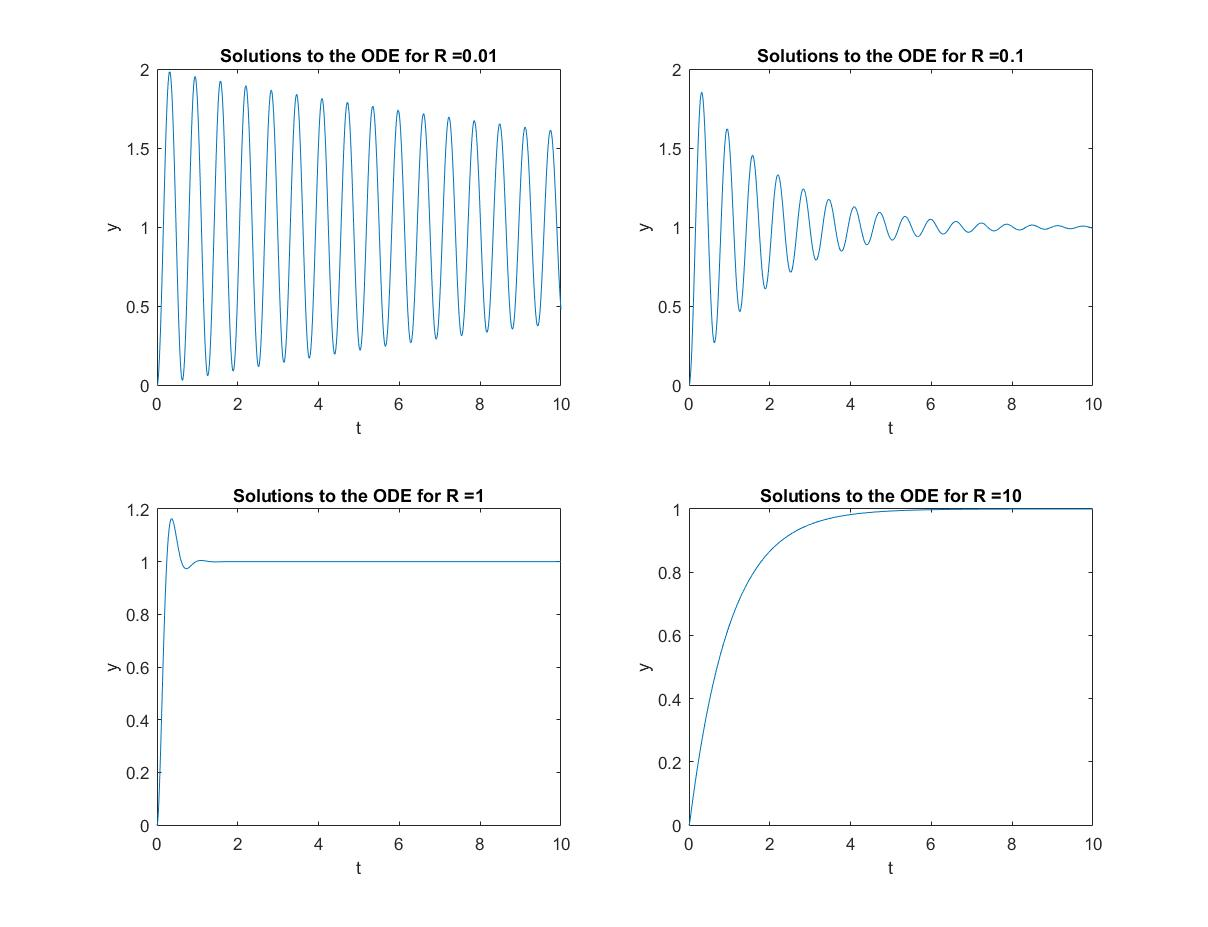
\includegraphics[width=\textwidth]{p1}
\caption{Plot of the solutions to the ODE for varying R}
\label{solplot1}
\end{figure}


\section*{C.1.1.2}
In this subtask the following differential equation is calculated.
\begin{equation}
\frac{d^3y}{dt^3}+3\frac{d^2y}{dt^2}+2\frac{dy}{dt}+Ky = 0,\quad y(0)=1,\quad \frac{dy}{dt}(0)=1,\quad \frac{d^2y}{dt^2}(0) = 1
\end{equation}

The desired solution is to rewrite the question in matrix form and it is done as follow. 
\begin{equation} \begin{aligned}
u_1 & = y \\ u_2 & = \dot{u_1} \\ u_3 & = \dot{u_2} \\
\dot{u_3} + 3u_3 + 2u_2 + Ku_1 & = 0 \\ 
& \Downarrow \\ 
\begin{bmatrix} \frac{du_1}{dt} \\ \frac{du_2}{dt} \\ \frac{du_3}{dt} \end{bmatrix} & = 
\begin{bmatrix} 0 & 1 & 0 \\ 0 & 0 & 1 \\ -K & -2 & -3 \\ \end{bmatrix} 
\begin{bmatrix} u_1 \\ u_2 \\ u_3 \end{bmatrix}
\end{aligned} \end{equation}

The numerical solutions with different $K$ were calculated with Matlab. The results are plotted as below. 

\begin{figure}[h]
\centering
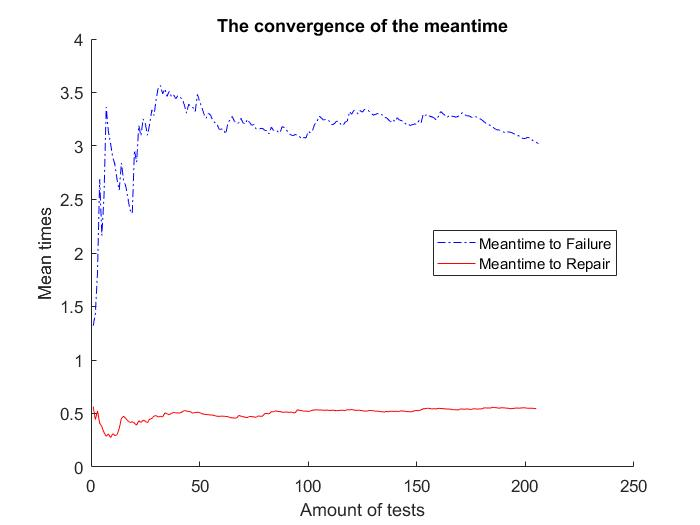
\includegraphics[width=\textwidth]{p2}
\caption{Plot of the solutions to the ODE for varying K.}
\label{solplot2}
\end{figure}

To further investigate the stability of the solution, the eigenvalues of the matrix A(K) can be plotted as K varies. The solution is unstable if some of the eigenvalues are located in the right half of the complex plane. A plot of the root locus for A(K) is shown in figure \ref*{rootlocus}.

\begin{figure}[h]
\centering
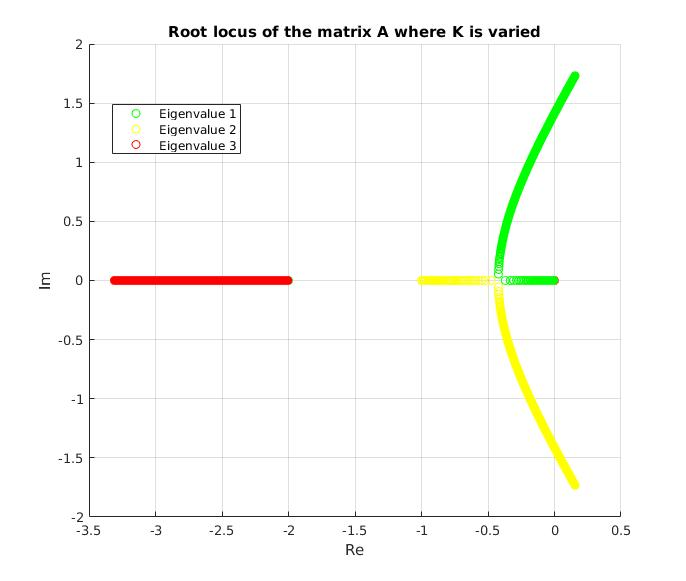
\includegraphics[width=\textwidth]{c112RL}
\caption{Root Locus of the matrix A.}
\label{rootlocus}
\end{figure}

Note the symmetry, it is clear that the system becomes unstable as two of the eigenvalues move into the right side of the complex plane. Computing the value for K for which this happens gives K=6.00. 

\section*{C.1.1.2.2}
In this subtask, the critical points of a nonlinear ODE system are analyzed. The ODE system is:
\begin{equation}
\begin{aligned}
\frac{du_1}{dt} & = 5u_1 + 4u_2 - u_1u_3 \\
\frac{du_2}{dt} & = u_1 + 4u_2 - u_2u_3 \\
\frac{du_3}{dt} & = u_1^2 + u_2^2 - 89 \\
\Downarrow \\
\dot{\vec{u}} & = \vec{f}(\vec{u})
\end{aligned}
\end{equation}

To calculate the critical points, the Newton's method was used. Thus the Jacobian matrix of the function $\vec{f}$ was calculated analytically and it is: 
\begin{equation}
\begin{aligned}
\vec{J}(\vec{u}) & = 
\begin{bmatrix}
5-u_3 & 4 & -u_1 \\
1 & 4-u_3 & -u_2 \\
2u_1 & 2u_2 & 0 \\
\end{bmatrix}
\end{aligned}
\end{equation}

Then the critical points can be calculated with the recursive formula below which is the Newton's method. 
\begin{equation}
\vec{u}^{(i+1)} = \vec{u}^{(i)}−(\vec{J}(\vec{u}^{(i)}))^{-1} \vec{f}(\vec{u}^{(i)})
\end{equation}

With Matlab and the initial guessing the following critical points are calculated.
\begin{equation}
\begin{aligned}
\vec{u}_1 & = [7.9446  , -5.0876  ,  2.4384] \\
\vec{u}_2 & = [-8.0000  ,  5.0000  ,  2.0000] \\
\vec{u}_3 & = [8.7881  ,  3.4309  ,  6.5616] \\
\vec{u}_4 & = [-8.7881 ,  -3.4309  ,  6.5616] 
\end{aligned}
\end{equation}

Stability of the critical points is given by either the eigenvalues of the Jacobian matrix at the critical points with a negative real part. The eigenvalues can be calculated easily with Matlab function $eig$. The results are:
\begin{equation}
\begin{aligned}
\\
   [0.0000 -13.3417i & \qquad  0.0000 +13.3417i & \quad  4.1231 + 0.0000i] \\
   [0.2344 -13.3350i & \qquad  0.2344 +13.3350i & \quad  4.5312 + 0.0000i] \\
   [0.0000 -13.3418i & \qquad  0.0000 +13.3418i & \quad -4.1232 + 0.0000i] \\
   [0.0000 -13.3418i & \qquad  0.0000 +13.3418i & \quad -4.1232 + 0.0000i] \\
\end{aligned}
\end{equation}
Then it is easy to see that the first two critical points are not stable and the last two are stable. 


\end{document}




\iffalse
%% KOD FÖR C1.1.2(del1)
clc,clear all, close all

%%Problem C1,1,2
pos=1;
for K=[0 1 4 8]
%Defining matrix

A= [ 0 1 0; 0 0 1; -K -2 -3];

u0=[ 1 1 1]'; t0 = 0;

h=0.1; N=1000;

result=[u0']; time=[t0];


for k = 1:N
    
   t=k*h;
   u=expm(A*t)*u0;
   result=[result;u'];
   time=[time;t];
end

subplot(2,2,pos)
plot(time,result)
pos=pos+1;
legend('y','dy/dt','dy^2/dt^2')



end 
\fi

%%
%% Root locus of A
figure
grid on
count=1;
for K=0:0.01:10
          A=[0 1 0; 0 0 1 ;-K -2 -3]';
  eigenvalue=eig(A);
    t=length(eigenvalue);
    hold on
   
   plot(real(eigenvalue(1)),imag(eigenvalue(1)),'go',real(eigenvalue(2)),imag(eigenvalue(2)),'yo',real(eigenvalue(3)),imag(eigenvalue(3)),'ro')
real_part=real(eigenvalue);



   %Finding K where system becomes unstable
 for i=1:3
   if real_part(i) > 0
       
       
      K_unstable(count) = K;
      count=count+1;
   end
    end
%unstable k
    
   %Finding K where system becomes unstable
end

   legend('Eigenvalue 1','Eigenvalue 2','Eigenvalue 3')
   ylabel('Im')
   xlabel('Re')
   title('Root locus of the matrix A where K is varied')

   
   Unstable_K=K_unstable(1)
